\chapter{Introduction}

\section{Caching Problem}

Storing data in a faster storage medium to serve future requests faster for that data is a 
very common technique in computer science called caching. We will consider the problem 
of caching of pages of fixed size in a buffer pool of fixed size.

We call cache hit when the requested page is already in the cache, and cache fault or miss
when the requested page is not in the cache. Generally, the goal is to maximize the number
of cache hits.

When a page is accessed, and the buffer is full, we need to decide which page to evict
from the cache to make space for the new page. This is called the cache eviction policy,
and it is a crucial part of the caching problem.

The optimal cache eviction policy is to evict the page that will be requested the farthest
in the future \cite{lecture-notes-1} \cite{lecture-notes-2} \cite{article-for-belady-ref-1}.
But this is impractical in most cases, since it is generally impossible to predict how
far in the future a page will be requested.

Several cache eviction policies have been developed, which incorporate information
about recency and/or frequency of page requests to make eviction decisions, we will
discuss some of them in detail in the following chapters.

\section{Buffer Sharing in Multi-Tenant Caches}

In a multi-tenant environment, multiple tenants share the same buffer pool. Proper 
allocation of the buffer pool among tenants is crucial for the performance of each
tenant workload \cite{buffer-sharing-1}.

In this thesis, we will consider the problem of buffer sharing in multi-tenant caches,
where each tenant has completely different workloads, data of one tenant is completely
independent of the data of another tenant.

We mainly consider small number of tenants, since it is common in possible applications, 
experiments have mainly 4 or 5 tenants, with some of them with up to 10 tenants, however, 
the proposed algorithms also work for larger number of tenants.

\subsection{Global, Static and Dynamic Buffer Allocation}

Some of the main approaches to buffer allocation in multi-tenant caches are:

\begin{enumerate}
    \item Global Buffer Allocation: All tenants share the same buffer pool, and the 
    buffer allocation is fixed. This approach is very simple and easy to implement,
    but it allows unlimited sharing of the buffer, and hence, it becoomes difficult to 
    guarantee the specified performance goal for individual tenants
    \cite{article-for-2level-forecasting} (Fig \ref{fig:figA-1}).
    \item Static Buffer Allocation: Each tenant has a fixed buffer size, and the buffer
    allocation is fixed. While straightforward to manage without sharing, a critical 
    downside of static caching is that it is hard to estimate the required amount of 
    the cache space in advance \cite{article-for-2level-forecasting} (Fig \ref{fig:figB-1}).
    \item Dynamic Buffer Allocation: The size of cache space for a tenant is adjusted 
    over time by monitoring performance. For this, it is critical to have good seasonality
    recommendations of cache sizes per tenant. Inadequate predictions will lead to the waste
    of resources or the failure of the performance guarantee \cite{article-for-2level-forecasting}
    There have been various studies to address this problem, such as based on the 
    approximation to concave functions \cite{approx-concave-functions} and a 
    learning-based prediction \cite{learning-based-prediction}, but it is still a 
    challenging problem to make accurate estimations of access patterns with an 
    acceptable error bound.
\end{enumerate}

\begin{figure}[H]
    \centering
    \begin{minipage}{0.4\textwidth}
        \centering
        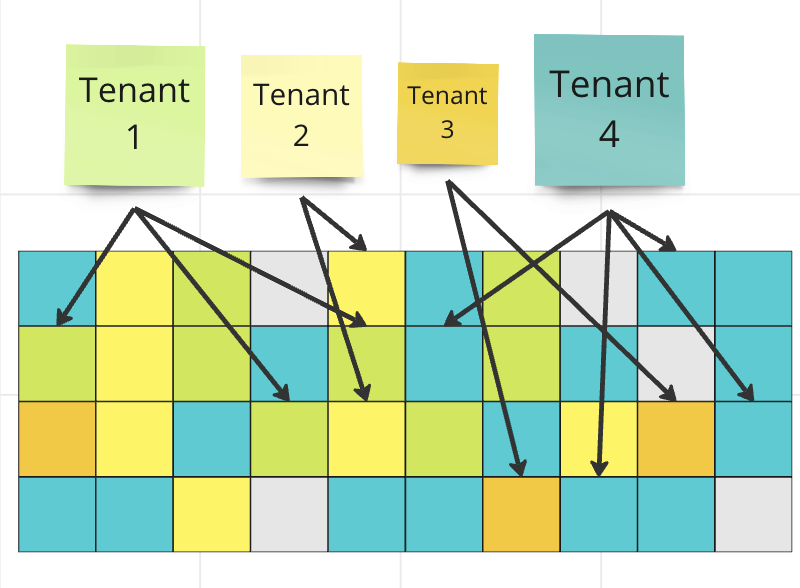
\includegraphics[width=\textwidth]{global_cache.png}
        \caption{Global Caching}
        \label{fig:figA-1}
    \end{minipage}
    \hfill
    \begin{minipage}{0.4\textwidth}
        \centering
        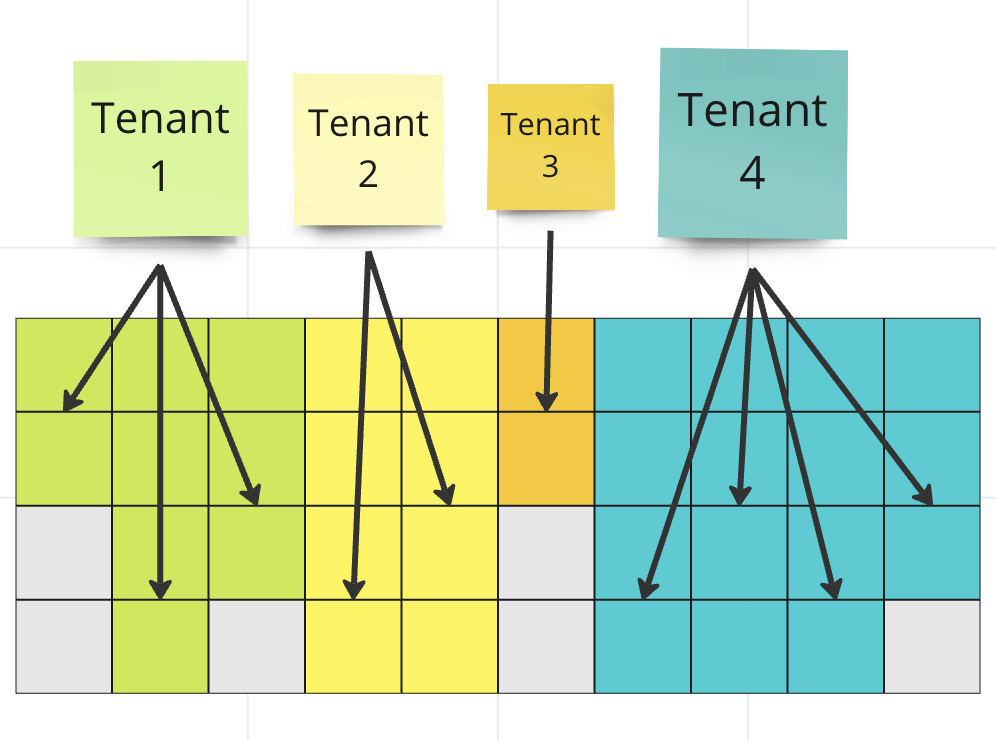
\includegraphics[width=\textwidth]{static_cache.png}
        \caption{Static Caching}
        \label{fig:figB-1}
    \end{minipage}
\end{figure}

The main case of study in this thesis is the dynamic buffer allocation, therefore our
caching policy will be adaptive to the buffer allocation of each tenant.

\subsection{Two level forecasting algorithm}

Since we are mainly interested in dynamic buffer allocation, caching problem in this
case can be seen as a two level forecasting problem. The first level is the seasonality
recommendation algorithm, which gives the buffer allocation of each tenant, and the
second level is the eviction policy, which makes eviction decisions based on the buffer
allocation.

The main focus of this thesis is on the eviction policy, for that, we will assume that
the buffer recommendations are given, and we will compare the performance of different
eviction policies.

While the recommendations are given, this does not mean that will have the cache problem
like single caches with fixed size, since the buffer allocation of each tenant is a 
recommendation that does not needs to be followed exactly, and it will also change
over time, therefore our eviction policy needs to be adaptive to the buffer allocation
of each tenant.

\subsection{Application to Multi-Tenant Relational Databases}

Relational database systems are widely used in many enterprises to store, manage and 
query data in applications in a structured way. Several commercial cloud relational
database services, such Google Cloud SQL \cite{google-cloud-sql}, Microsoft Azure SQL 
Database \cite{azure-sql}, and Oracle Cloud Database \cite{oracle-cloud} have emerged. 

In this cloud services, multi tenancy is crucial to increase consolidation and reduce
cost by sharing resources among tenants \cite{buffer-sharing-1}.

A database as a service (DaaS) provider would like to overbook the resources, i.e. 
promise more resources to tenants in aggregate than is physically available on the
machine, yet without affecting tenant performance. This is based on the observation 
that at any point in time some tenants on the machine are likely to use much fewer 
resources than they are promised. \cite{buffer-sharing-1} The main challenge is to 
allocate resources to tenants in a way that guarantees the performance of each tenant 
workload.

\section{Service Level Agreements and Hit Ratio Degradation}

In a multi-tenant environment, it is common to have service level agreements (SLAs)
or Quality of Service (QoS) requirements for each tenant. For example, in a cloud 
database service, a tenant may have promosed some amount of buffer space, and the
provider should guarantee a performance goal for the tenant.

The performance goal can be defined in terms of fault or hit ratio, like the fault
or hit ratio achieved if the tenant would had a dedicated cache of some promised size.
In a case where there is not a promised size like in the cloud environment, we can 
compare the achieved hit ratio with the hit ratio achieved by a tenant with a dedicated
cache of the size of the recommendation we have.

Metrics comparing the achieved hit ratio with the hit ratio of a dedicated cache have
been proposed in the literature, like the hit ratio degradation (HRD), as the difference 
in total hits, between the baseline and any scheme that assigns memory dynamically, 
normalized by the total memory accesses \cite{buffer-sharing-1} or other quality of 
service metrics like in \cite{learning-based-prediction}.

\section{Minimum and Maximum Buffer Sizes}

Since our main focus is dynamic buffer allocation, we will also define minimum and maximum 
buffer sizes for each tenant, to guarantee a minimum performance goal for each tenant, and
to avoid tenants taking too much buffer space.

This approach was used in ICPC 2023 Online Spring Challenge powered by Huawei: Buffer Sharing in 
Multi-Tenant Database Environment \cite{huawei-challenge}.

Minimum and maximum buffer sizes can be defined based on the buffer size recommendations per tenant,
for example, the minimal buffer size can be 40\% of the recommendation, and the maximal buffer size
can be 250\% of the recommendation.

\section{Penalty Function Optimization}

We will consider the following penalty function to optimize:

$$
\sum_{t \in \text{Tenants}} \left( \frac{\text{Solution Cache faults}_t - \text{LRU Cache faults}_t}{\text{LRU Cache faults}_t} \right) ^2 \text{Priority}_t \left[\text{Solution Cache faults}_t \geq \text{LRU Cache faults}_t\right]
$$

In which, for each tenant $t$:
\begin{itemize}
    \item $\text{Solution Cache faults}_t$ is the number of cache faults of the eviction policy we are testing.
    \item $\text{LRU Cache faults}_t$ is the number of cache faults of the LRU eviction policy if we had a dedicated cache of some promised size.
    \item $\text{Priority}_t$ is the priority of the tenant, which can be defined in terms of the cost of a cache fault for the tenant, or the importance of the tenant. If there is no need to prioritize tenants, we can set $\text{Priority}_t = 1$ for all tenants, in case it is needed, priorities can be defined based on how importanat is for each tenant to achieve the promised hit ratio.
    \item The term in brackets is a condition so we only penalize the eviction policy if it has more cache faults than the isolated LRU eviction policy.
\end{itemize}

We normalize by the number of cache faults of the isolated LRU eviction policy, to make 
the penalty function independent of the number of tenants and the size of the cache, and to 
not prioritize tenants by the size of the access pattern.

We use squared ratio to penalize more the eviction policies that have a higher difference
in cache faults with the isolated LRU eviction policy, since we want to minimize the
difference in cache faults with the isolated LRU eviction policy, and smaller differences
are more tolerable.

This cost function was also used in ICPC 2023 Online Spring Challenge powered by Huawei: 
Buffer Sharing in Multi-Tenant Database Environment \cite{huawei-challenge}. Better results
were observed using this penalty function instead of using cache hits instead of faults.

Our goal is to minimize the penalty function, and we will compare the performance of
different eviction policies based on this penalty function.

\section{Research Question}

In multi-tenant caches, the main challenges are to allocate the buffer space among tenants
in a way that guarantees the performance of each tenant workload, and to design an eviction
policy that best satisfies the service level agreements for each tenant and does not waste
buffer space. 

Improving the cache performance in multi-tenant caches is interesting both for commercial
and research purposes, and it results in the main research question of this thesis:

\textit{How to design an eviction policy for multi-tenant caches that best satisfies 
the service level agreements for each tenant and does not waste buffer space?}

\section{Objectives}

To address the research question, the following objectives are proposed:

\begin{enumerate}
    \item Provide a clear overview of the multi-tenant caching problem.
    \item Describe the baseline algorithm with tenant selection policy and the cache eviction algorithm.
    \item Implement and describe different eviction policies, adapting them to the dynamic buffer size of each tenant.
    \item Perform experiments with real world data to compare the performance of different eviction policies.
    \item Analyze the results and propose improvements to the tenant selection and eviction policies.
\end{enumerate}

\section{Outline}

The outline for the rest of the thesis is as follows:

\begin{itemize}
    \item \textbf{Chapter 2: Algorithm Overview} - Will describe the base algorithm that we used, and discuss possible tenant selection and cache eviction policies.
    \item \textbf{Chapter 3: Experiments and Methodology} - Will describe the datasets we used, with data collection and processing part, and the performed experiments.
    \item \textbf{Chapter 4: Results} - Will present and analyze the results of the experiments, comparing different eviction policies.
    \item \textbf{Chapter 5: Conclusions and Recommendations} - Will summarize the results and propose recommendations for future work.
\end{itemize}